% Présentation des principales versions imprimées et du Textus Receptus.

\documentclass[11pt]{beamer}
\graphicspath{{img/}{./}}
\usepackage[french]{babel}
\usepackage{graphicx}
\usepackage{ulem} %Pour biffer du texte \sout{texte barré}
\usepackage{xcolor} 
\usepackage{tabularx}
\usepackage{parallel}
%\usepackage[babelshorthands]{polyglossia}
\usepackage{ragged2e} 


%Allignemebnt droite/gauche
\usepackage{polyglossia}
%\usepackage[babelshorthands]{polyglossia} %[babelshorthands] permet d'avoir les guillemets allemands avec le code "`toto"' et les guillemets français avec le code "<tata">


\usepackage{multirow} 
\setmainlanguage{english}
\usepackage[autostyle]{csquotes}
\MakeOuterQuote{"}
\DeclareQuoteStyle{english}%
    {\textquotedblleft}
    [\textquotedblleft]
    {\textquotedblright}
        [0.05em]
    {\textquoteleft}
    [\textquoteleft]
    {\textquoteright}
% \DeclareQuoteStyle[quotes]{french}
%   {\mkfrenchopenquote{«}}
%   {\mkfrenchclosequote{\nobreakspace»}}
%   {\textquotedblleft}
%   {\textquotedblright}
% \DeclareQuoteStyle[quotes*]{french}
%   {\mkfrenchopenquote{«}}
%   {\mkfrenchclosequote{\nobreakspace»}}
%   {\mkfrenchopenquote{\textquotedblleft}}
%   {\mkfrenchclosequote{\textquotedblright}}
% \DeclareQuoteStyle[guillemets]{french}
%   [\initfrenchquotes]
%   {\mkfrenchopenquote{«}}
%   [\mkfrenchopenquote{«}]
%   {\mkfrenchclosequote{\nobreakspace»}}
%   {\mkfrenchopenquote{«}}
%   [\mkfrenchopenquote{«}]
%   {\mkfrenchclosequote{\nobreakspace»}}
% \DeclareQuoteStyle[guillemets*]{french}
%   [\initfrenchquotes]
%   {\mkfrenchopenquote{«}}
%   [\mkfrenchopenquote{\nobreakspace»}]
%   {\mkfrenchclosequote{\nobreakspace»}}
%   {\mkfrenchopenquote{«}}
%   [\mkfrenchopenquote{\nobreakspace»}]
%   {\mkfrenchclosequote{\nobreakspace»}}




\setotherlanguage{greek}
\newfontfamily\greekfont[Script=Greek]{Linux Libertine O}
\newfontfamily\greekfontsf[Script=Greek]{Linux Libertine O}
\setotherlanguage{hebrew}
\newfontfamily{\hebrewfont}[Script=Hebrew, Path=./fonts/]{SBL_Hbrw.ttf}
\newfontfamily{\hebrewfontsf}[Script=Hebrew]{Miriam CLM}
\newfontfamily{\hebrewfonttt}[Script=Hebrew]{Miriam Mono CLM}
\setotherlanguage{syriac}
\newfontfamily\syriacfont[Script=Syriac, Path=./fonts/]{EstrangeloEdessa.ttf}

\usepackage{booktabs} % Allows the use of \toprule, \midrule and \bottomrule for better rules in tables
%% Allow the use of tcolorbox
\usepackage[skins]{tcolorbox}
%\usetheme{default}
%\usetheme{AnnArbor}
%\usetheme{Antibes}
%\usetheme{Bergen}
%\usetheme{Berkeley}
%\usetheme{Berlin}
%\usetheme{Boadilla}
%\usetheme{CambridgeUS}
%\usetheme{Copenhagen}
%\usetheme{Darmstadt}
%\usetheme{Dresden}
%\usetheme{Frankfurt}
%\usetheme{Goettingen}
%\usetheme{Hannover}
%\usetheme{Ilmenau}
\usetheme{JuanLesPins}
%\usetheme{Luebeck}
%\usetheme{Madrid}
%\usetheme{Malmoe}
%\usetheme{Marburg}
%\usetheme{Montpellier}
%\usetheme{PaloAlto}
%\usetheme{Pittsburgh}
%\usetheme{Rochester}
%\usetheme{Singapore}
%\usetheme{Szeged}
%\usetheme{Warsaw}

%----------------------------------------------------------------------------------------
%	SELECT COLOR THEME
%----------------------------------------------------------------------------------------

% Beamer comes with a number of color themes that can be applied to any layout theme to change its colors. Uncomment each of these in turn to see how they change the colors of your selected layout theme.

%\usecolortheme{albatross}
%\usecolortheme{beaver}
%\usecolortheme{beetle}
%\usecolortheme{crane}
%\usecolortheme{dolphin}
%\usecolortheme{dove}
%\usecolortheme{fly}
%\usecolortheme{lily}
%\usecolortheme{monarca}
%\usecolortheme{seagull}
%\usecolortheme{seahorse}
%\usecolortheme{spruce}
%\usecolortheme{whale}
%\usecolortheme{wolverine}

%----------------------------------------------------------------------------------------
%	SELECT FONT THEME & FONTS
%----------------------------------------------------------------------------------------
\setmainfont{cochineal}
% Beamer comes with several font themes to easily change the fonts used in various parts of the presentation. Review the comments beside each one to decide if you would like to use it. Note that additional options can be specified for several of these font themes, consult the beamer documentation for more information.

%\usefonttheme{default} % Typeset using the default sans serif font
\usefonttheme{serif} % Typeset using the default serif font (make sure a sans font isn't being set as the default font if you use this option!)
%\usefonttheme{structurebold} % Typeset important structure text (titles, headlines, footlines, sidebar, etc) in bold
%\usefonttheme{structureitalicserif} % Typeset important structure text (titles, headlines, footlines, sidebar, etc) in italic serif
%\usefonttheme{structuresmallcapsserif} % Typeset important structure text (titles, headlines, footlines, sidebar, etc) in small caps serif

%------------------------------------------------

%\usepackage{mathptmx} % Use the Times font for serif text
%\usepackage{palatino} % Use the Palatino font for serif text


%\usepackage{helvet} % Use the Helvetica font for sans serif text
%\usepackage[default]{opensans} % Use the Open Sans font for sans serif text
%\usepackage[default]{FiraSans} % Use the Fira Sans font for sans serif text
%\usepackage[default]{lato} % Use the Lato font for sans serif text

%----------------------------------------------------------------------------------------
%	SELECT INNER THEME
%----------------------------------------------------------------------------------------

% Inner themes change the styling of internal slide elements, for example: bullet points, blocks, bibliography entries, title pages, theorems, etc. Uncomment each theme in turn to see what changes it makes to your presentation.

%\useinnertheme{default}
%\useinnertheme{circles}
\useinnertheme{rectangles}
%\useinnertheme{rounded}
%\useinnertheme{inmargin}

%----------------------------------------------------------------------------------------
%	SELECT OUTER THEME
%----------------------------------------------------------------------------------------

% Outer themes change the overall layout of slides, such as: header and footer lines, sidebars and slide titles. Uncomment each theme in turn to see what changes it makes to your presentation.

%\useoutertheme{default}
%\useoutertheme{infolines}
%\useoutertheme{miniframes}
%\useoutertheme{smoothbars}
%\useoutertheme{sidebar}
%\useoutertheme{split}
%\useoutertheme{shadow}
%\useoutertheme{tree}
%\useoutertheme{smoothtree}

%\setbeamertemplate{footline} % Uncomment this line to remove the footer line in all slides
%\setbeamertemplate{footline}[page number] % Uncomment this line to replace the footer line in all slides with a simple slide count

%\setbeamertemplate{navigation symbols}{} % Uncomment this line to remove the navigation symbols from the bottom of all slides
\usepackage[style=sbl]{biblatex}


\DeclareSourcemap{
  \maps[datatype=bibtex]{
    \map{
      \step[fieldset=doi, null]
      \step[fieldset=language, null]
      \step[fieldset=issn, null]{}
      \step[fieldset=url, null]{}
      \step[fieldset=isbn, null]{}
      \step[fieldset=eprint, null]{}
    }
  }
}

\addbibresource{references.bib}
%\defbibheading{bibempty}{}

%----------
% Define sectioning
\AtBeginSection[]{
  \begin{frame}
  \vfill
  \centering
  \begin{beamercolorbox}[sep=8pt,center,shadow=true,rounded=true]{title}
    \usebeamerfont{title}\insertsectionhead\par%
  \end{beamercolorbox}
  \vfill
  \end{frame}
}

%-----------

%----------------------------------------------------------------------------------------
%	PRESENTATION INFORMATION
%----------------------------------------------------------------------------------------


\title{Introduction à la critique textuelle}
\author[Frédérique Michèle Rey, Sophie Robert-Hayek]{Frédérique Michèle Rey \& Sophie Robert-Hayek}


\institute[UL]{Université de Lorraine } %\smallskip \textit{frederique.rey@univ-lorraine.fr / sophie.robert@univ-lorraine.fr}}

\date{}
\setbeamertemplate{footline}[frame number]

\usepackage[table]{xcolor}
\usepackage[dvipsnames]{xcolor}
\usepackage{forest}
\usepackage{tikz-qtree}
\usepackage[font=scriptsize]{caption}
\begin{document}
\title{Le texte imprimé du Nouveau Testament}
\subtitle{Critique textuelle du Nouveau Testament}

\begin{frame}{}
    \titlepage
\end{frame}

\begin{frame}{Plan du cours}
\tableofcontents
\end{frame}

\section{Les premières bibles imprimées}

\begin{frame}
  \frametitle{L'invention de l'imprimerie}
  \begin{alertblock}{}
      Au milieu du XVe siècle, le monde de la littérature a été révolutionné par l'invention de l'imprimerie : pour la première fois dans le monde occidental, il est devenu possible de \textbf{reproduire un document en un nombre illimité d'exemplaires identiques}.
  \end{alertblock}
  La presse à imprimer marque le début d'une nouvelle ère où les livres ne dépendent plus des manuscrits copiés à la main.
\centering
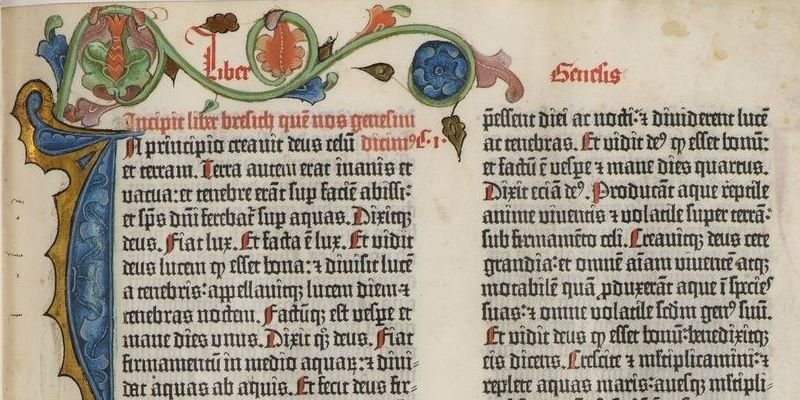
\includegraphics[width=0.5\linewidth]{img/incipit_genese_image_en_une.jpg}
\end{frame}



\begin{frame}{La Polyglotte Complutensienne}
    \begin{alertblock}{}
        Entre 1502 et 1522 est préparée la \textit{Polyglotte Complutensienne} (d'Alcala), 
        Bible polyglotte complète, ainsi que la première version \textbf{imprimée} du Nouveau Testament en grec, de la Septante et du Targoum Onkelos.
    \end{alertblock}
    Mais la publication fut postérieure à l'impression, et celle-ci est finalement publiée en 1522...!
\end{frame}


\begin{frame}
  \frametitle{Le Nouveau Testament d'Érasme}
  \begin{alertblock}{}
      Dans une course contre l'imprimeur espagnol, Erasme prépare de 1515 à 1516 un Nouveau Testament Grec à l'aide de 6 manuscrits \textbf{byzantins}.
  \end{alertblock}

  Au cours des quatre révisions successives, le texte d'Erasme reste \textbf{hasardeux} et n'est que \textbf{très peu complété de témoins additionnels}.
\end{frame}


\section{Les éditions protestantes et le textus receptus}

\begin{frame}
  \frametitle{Le Nouveau Testament de Stephanus}
\begin{alertblock}{}
    \textbf{Robert Estienne} (\textbf{Stephanus}) est un imprimeur parisien et genevois, responsable de quatre éditions du Nouveau Testament en grec, à la base de la complutensienne, Erasme et 15 manuscrits additionnels.
\end{alertblock}
Pour la première fois, ses éditions :
\begin{itemize}
    \item Incluent l'apparat critique des manuscrits consultés et de la complutensienne;
    \item Incluent les divisions en verset.
\end{itemize}
\begin{block}{}
Théodore de Bèze publie à la suite neuf éditions du Nouveau Testament (1565-1604), se basant sur Erasme et sur Stephanus.
\end{block}
\end{frame}


\section{La naissance de la théologie du Textus Receptus}

\begin{frame}
  \frametitle{Le Textus Receptus}

Bonaventure et Abraham Elzevir (Pays-Bas) publient sept éditions du Nouveau Testament grec entre 1624 et 1678, \textbf{basés sur Stephanus et de Bèze}.

\begin{exampleblock}{}
\textbf{Textum} ergo habes, nunc ab \textbf{omnibus receptum}: in quo nihil immutatum aut corruptum damus. \\
\textit{Vous avez donc le texte maintenant accepté par tous : dans lequel nous ne donnons rien d'altéré ni de corrompu.}
\end{exampleblock}
  Le \emph{Textus Receptus} est le qualificatif encore utilisé pour parler de la troisième édition de Stephanus (1550) et la deuxième édition d'Elzevir (1633).
\end{frame}


\begin{frame}
  \frametitle{Le Textus Receptus}
    \begin{itemize}
        \item Le texte de la Vulgate est remplacé par ce texte pour devenir \textbf{normatif dans le protestantisme} (pendant près de 2 siècles et l'est toujours dans certains mouvements!);
        \item Principalement byzantin;
        \item Avec peu de bases philologiques (témoins choisis aléatoirement, pas de systématisation dans le choix de variants \dots).
    \end{itemize}
\end{frame}

\section{La chute du Textus Receptus}

\begin{frame}{L'accumulation des manuscrits}
\begin{alertblock}{}
    Du 17\ieme{} au 19\ieme{} siècle, un ensemble de témoins plus anciens que les Byzantins sont découverts et transcrits, et \textbf{un mouvement de critique générale envers le TR naît}
\end{alertblock}
\begin{itemize}
    \item \textbf{Lachmann} en 1842-50 propose une \textbf{toute nouvelle édition du texte néo-testamentaire};
    \item \textbf{Constantin von Tischendorf} (re)-découvre de nombreux manuscrits et édite huit éditions critiques (1841-1872);
    \item \textbf{Wescott et Hort} publient \textit{The New Testament in the Original Greek}, et systématisent des notions telles que celles du type de texte.
    \item \textbf{Hermann von Soden} propose de nouvelles théories de transmission du texte néo-testamentaire.
\end{itemize}
\end{frame}

\begin{frame}{La fin du Textus Receptus}
\begin{alertblock}{}
       Le milieu du 19\ieme{} siècle voit donc la fin d'une croyance en la supériorité du \texit{Textus Receptus}, et le naissance de la nouvelle ère de la \textbf{critique textuelle néo-testamentaire}. 
\end{alertblock}
\end{frame}

\begin{frame}{Questions}
    Questions ?
\end{frame}

\end{document}

